This chapter briefly introduces the basic concepts relative to physics engines, such as collision detection and constraints modelling. The purpose is to have the necessary background information to make the right choices later on.

\section{Problem statement}
Physics engines are used to simulate classical Newtonian mechanics in a computer. They model how objects accelerate, move and react to collisions with other objects. They also model how objects can be constrained to each other, for example with a hinge, and how it affects their movements. We restrict ourselves to the simulation of rigid bodies, which is a significant simplification of the problem since rigid bodies are idealized solid objects which never change shape.

\section{Major components of a physics engine}
The section is a summary of Jan Bender, Kenny Erleben, Jeff Trinkle and Erwin Coumans' work in \cite{BETC2012}. We will explain the key elements of rigid body physics simulation that we need to know in order to orient our work in the later chapters: collisions, the physics model and how it is integrated in time to produce a simulation.

\subsection{Collision detection \label{sec:collision}}
Collision detect is broken into three phases called the \emph{broad phase}, the \emph{mid phase} and the \emph{narrow phase}, as represented in \Cref{fig:star_collision}.

\begin{figure}
	\centering
	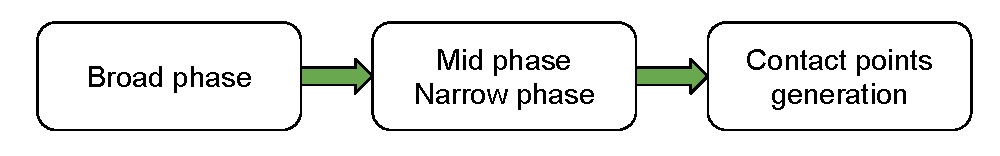
\includegraphics[width=0.9\textwidth]{figures/STAR_collision_v2}
	\caption[Collision detection]{Modular description of the collision detection in a physics engine. The mid and narrow phases are grouped together because they are often combined for performance reasons.}
	\label{fig:star_collision}
\end{figure}

During the broad phase, objects are approximated by simple geometric primitives as distances between such shapes are easy to compute. It is common to use spheres: if the distance between them is greater than the sum of their radii then the objects most certainly do not collide.

When an object has a complex shape, an additional phase called the mid phase separates the object into several simpler shapes to detect collisions. Finally the narrow phase uses the exact geometries of the object to find the contact points. These are then used in the collision resolution part of the simulation loop.

We do not need to dwell on collision detection longer than we already have. For our foreseen application it is sufficient to know that simpler shapes are easier to handle. For further discussion, different possible implementations are detailed in \cite{jimenez20013d}.

\subsection{Collision resolution \label{sec:contact}}
When bodies collide, high forces of very short duration are exerted. In the case of rigid bodies the duration is infinitesimal and as a consequence the forces become infinite. This is problematic because the simulator integrates forces to obtain velocities and positions: an infinite force would break the simulation loop.

A solution to this was proposed by Brian Mirtich in \cite{mirtich1996impulse}. The idea is to use the standard integration rule of the simulator up to the collision, use an impulse-momentum based collision rule to determine the velocities after impact and then resume the integration.

Several collision rules exist. One of them is called Newton's Hypothesis and it states that
\begin{align*}
	\mathbf{v}_n^+ & = e\mathbf{v}_n^-
\end{align*}
where $\mathbf{v}_n^+$ is the relative normal velocity after impact, $\mathbf{v}_n^-$ is the relative normal velocity before impact and $e \in [0, 1]$ is called the coefficient of restitution. When $e=1$ the collision is perfectly elastic and when $e=0$ all the energy is lost.

\subsection{Physics model}
The model is based on the three laws of Newton:
\begin{itemize}
	\item The velocity of an object remains unchanged if no force act upon it.
	\item The rate of change of the momentum of an object is equal to the force acting on it.
	\item For every force there is an equal and opposite force.
\end{itemize}

Physics engines usually represent positions, orientations and velocities in an inertial frame, which is a requirement for the laws of Newton to be true: 
\begin{itemize}
	\item Position is given by a vector $\mathbf{p} \in \mathcal{R}^3$, to represent the three translational degrees of freedom (DOF).
	\item Orientation can be represented either by rotation matrices or unit quaternions, the latter being usually preferred. A unit quaternion is four numbers $[Q_s, Q_x, Q_y, Q_z]$ constrained so that the number of their squares is one. $Q_s$ is computed in terms of the other numbers, so we correctly represent the three rotational DOF.
	\item Translational velocity is given by a vector $\mathbf{v} \in \mathcal{R}^3$. It should be noted that when the body rotates this vector only describes the translational velocity of the reference point of the body, which is usually chosen to be the centre of mass.
	\item Rotational velocity is given by a vector $\boldsymbol{\omega} \in \mathcal{R}^3$.
\end{itemize}
We define $\mathbf{q} = [\mathbf{p}^T, \mathbf{Q}^T]$ as the tuple containing the position of the COM and the orientation of a rigid body and $\mathbf{u} = [\mathbf{v}^T, \mathbf{w}^T]$ as its generalized velocity. When using quaternions, the velocity kinematic equations of a rigid body, i.e. the equations that relate $\mathbf{q}$ to $\mathbf{u}$ are:

\begin{align}
	\dot{\mathbf{q}} &= H\mathbf{u} \label{eq:kinematic}\\
	H &= \left(\begin{array}{c c}
		\mathbf{I}_{(3\times3)} & 0\\
		0 & \mathbf{G} \\
	\end{array}\right)\\
	\mathbf{G} &= \frac{1}{2}\left(\begin{array}{r r r}
		-Q_x & -Q_y & -Q_z \\
		Q_s  & Q_z  & Q_y  \\
		-Q_z & Q_s  & Q_x  \\
		Q_y  & -Q_x & Q_s
	\end{array}\right)\\
\end{align}
where $\mathbf{I}_{(3\times3)}$ is the 3-by-3 identity matrix.

Applying the second law of Newton to both translational and rotational forces produces what are called the Newton-Euler equations:
\begin{align}
m\dot{\mathbf{v}} &= \mathbf{f} \label{eq:newton1}\\
\mathbf{I}\dot{\boldsymbol{\omega}} + \boldsymbol{\omega} \times \mathbf{I}\boldsymbol{\omega} &= \boldsymbol{\tau} \label{eq:newton2}
\end{align}
where $\mathbf{I}$ is the \emph{inertia} of the object. It represents the tendency of an object to rotate around an axis. $\boldsymbol{\tau}$ is the \emph{torque} and represents the tendency of a force to rotate an object around an axis. It is defined as the cross product ($\times$) of a force vector and the vector of the distance between that force and the point of fixation of the rigid body. These equations express the relationship between forces acting on a rigid body and its velocity.

\Cref{eq:kinematic}, \Cref{eq:newton1} and \Cref{eq:newton2} are the basis of the physics model. Alone, they are sufficient to model the behaviour of a free falling rigid body. To handle collisions and constraints we must add equations that express different types of constraints : non-penetration of bodies, friction forces act in the direction that will most quickly stop the sliding and many others. 

All these equations form a differential non-linear complementarity problem (dNCP) that cannot be solved in closed form. It is thus discretized in time producing a series of non-linear complementarity problems (NCPs) whose solutions are an approximation of the state of the system. These solutions are usually found by linearising the NCP into a linear complementarity problem (LCP) to take advantage of the rich background for that type of problems. 
%
%\begin{figure}[htp]
%\centering
%\begin{subfigure}[b]{0.45\textwidth}
%	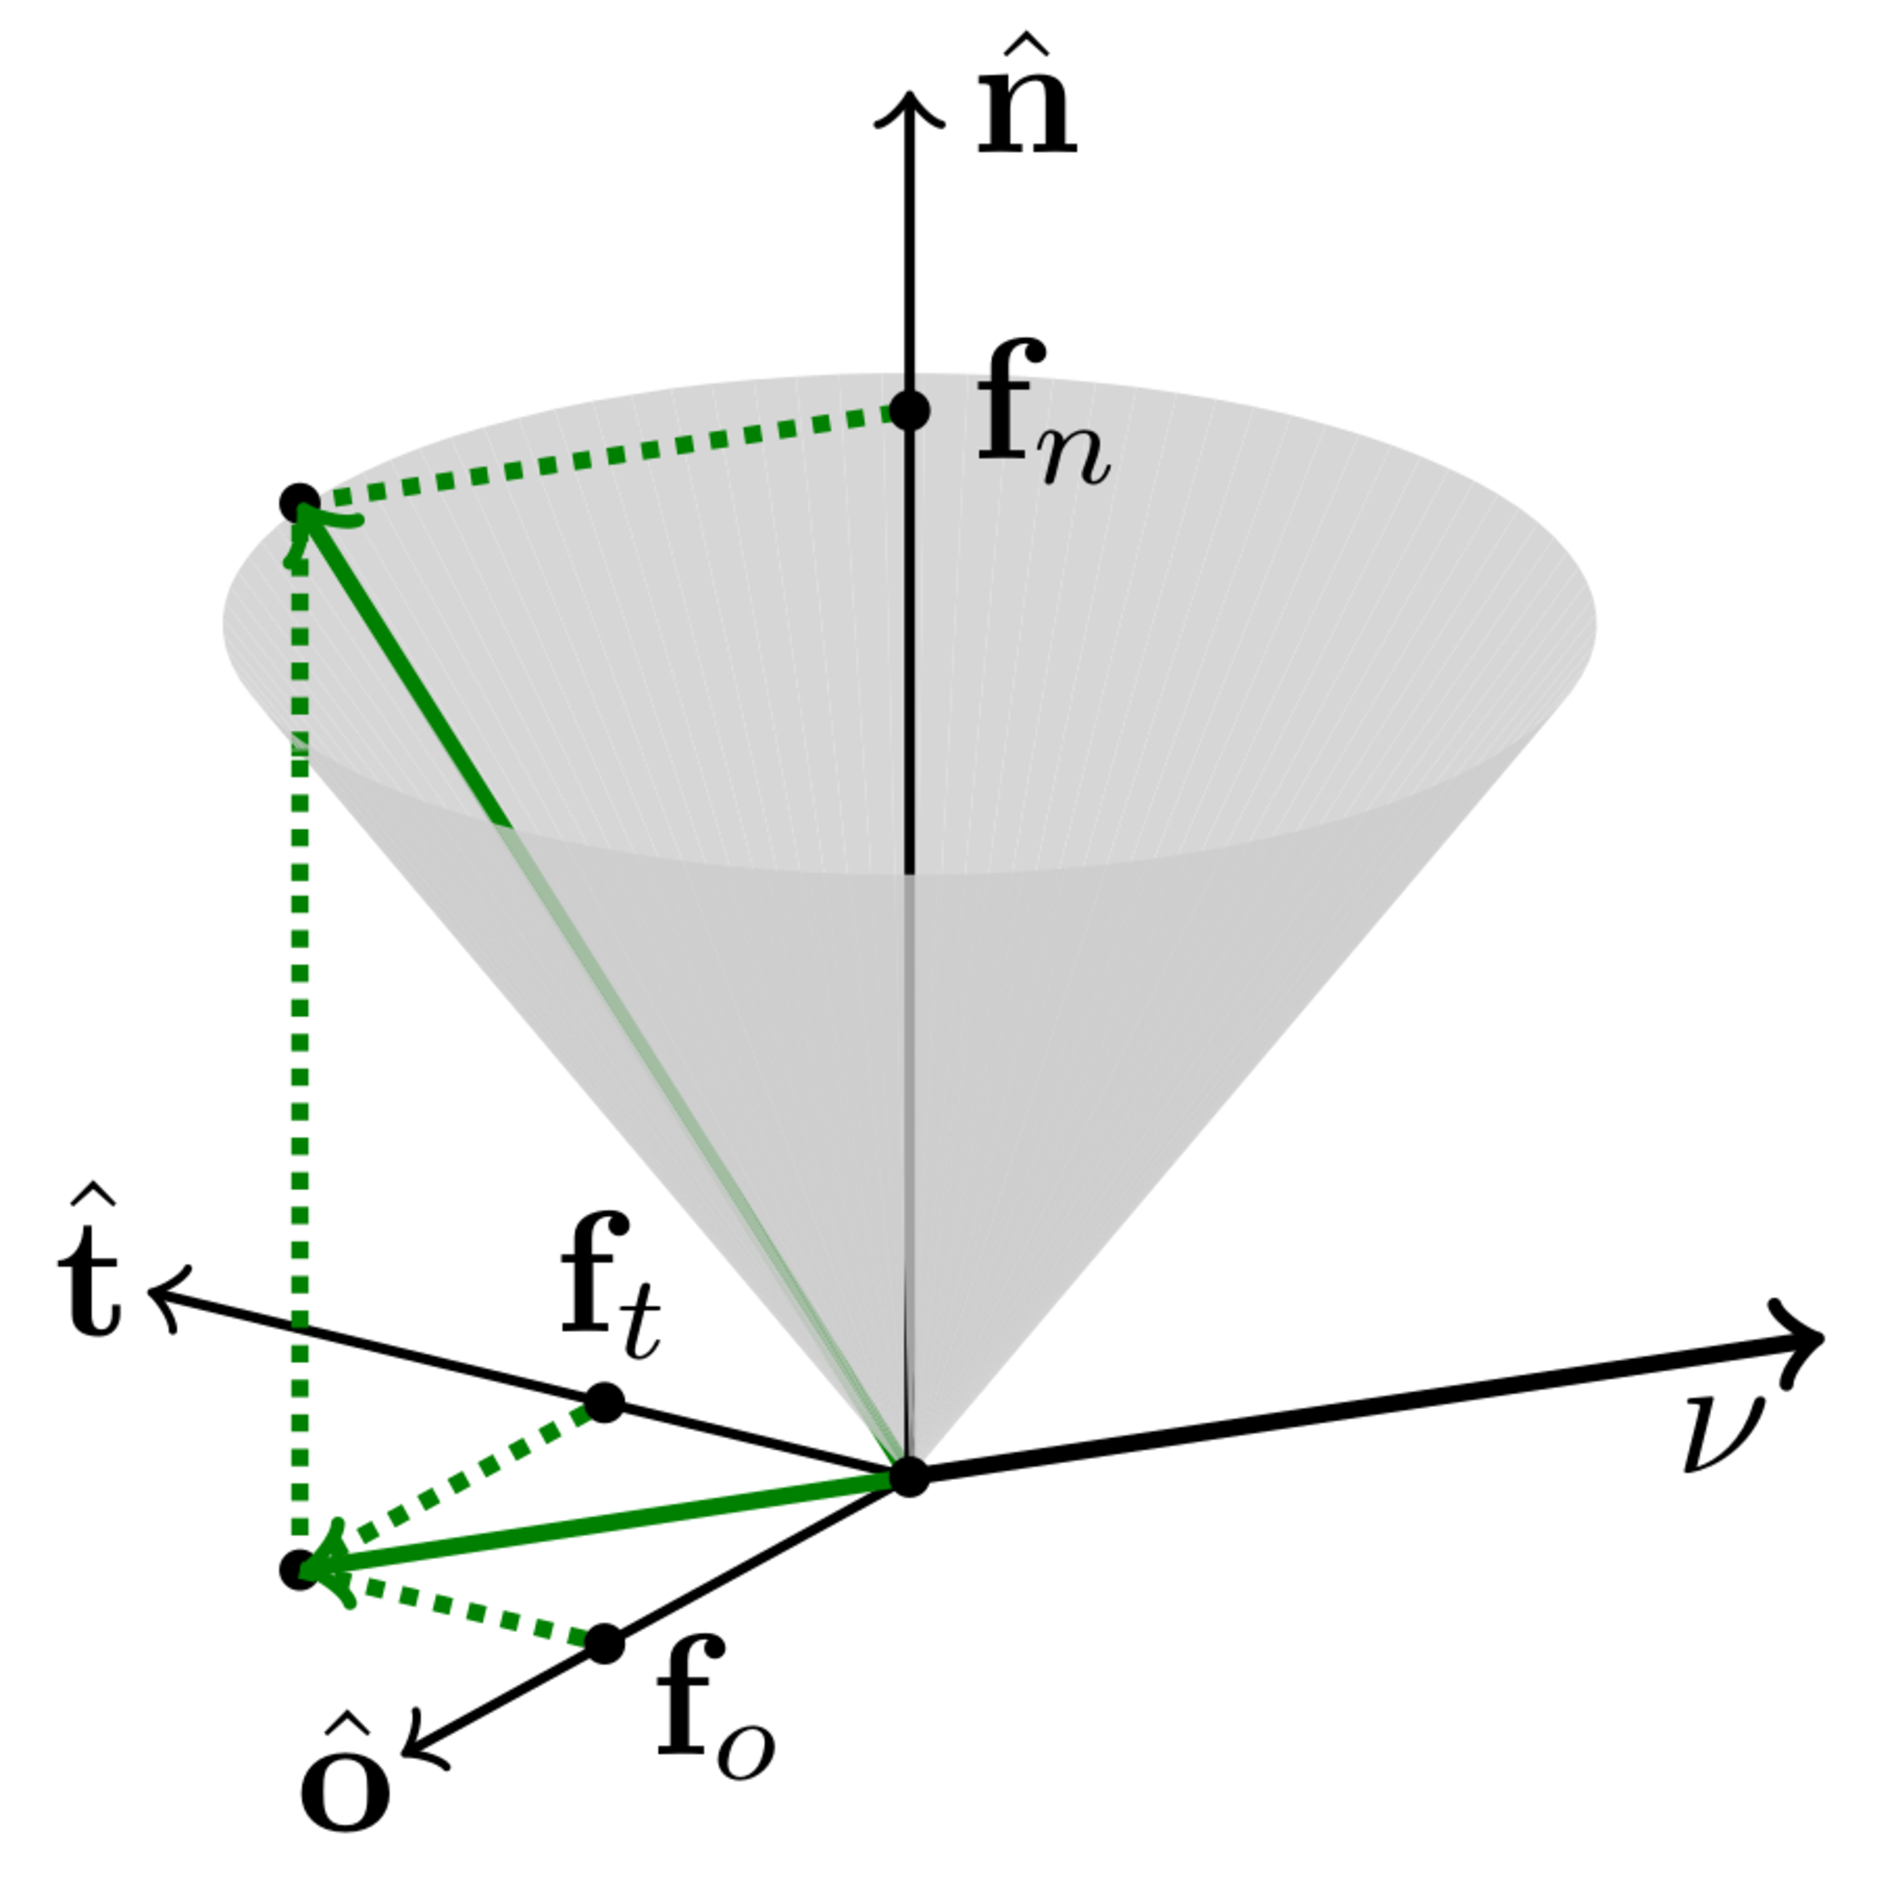
\includegraphics[width=\textwidth]{figures/friction_cone}
%	\caption{A friction cone}
%	\label{fig:friction_cone}
%\end{subfigure}
%\hfill
%\begin{subfigure}[b]{0.47\textwidth}
%	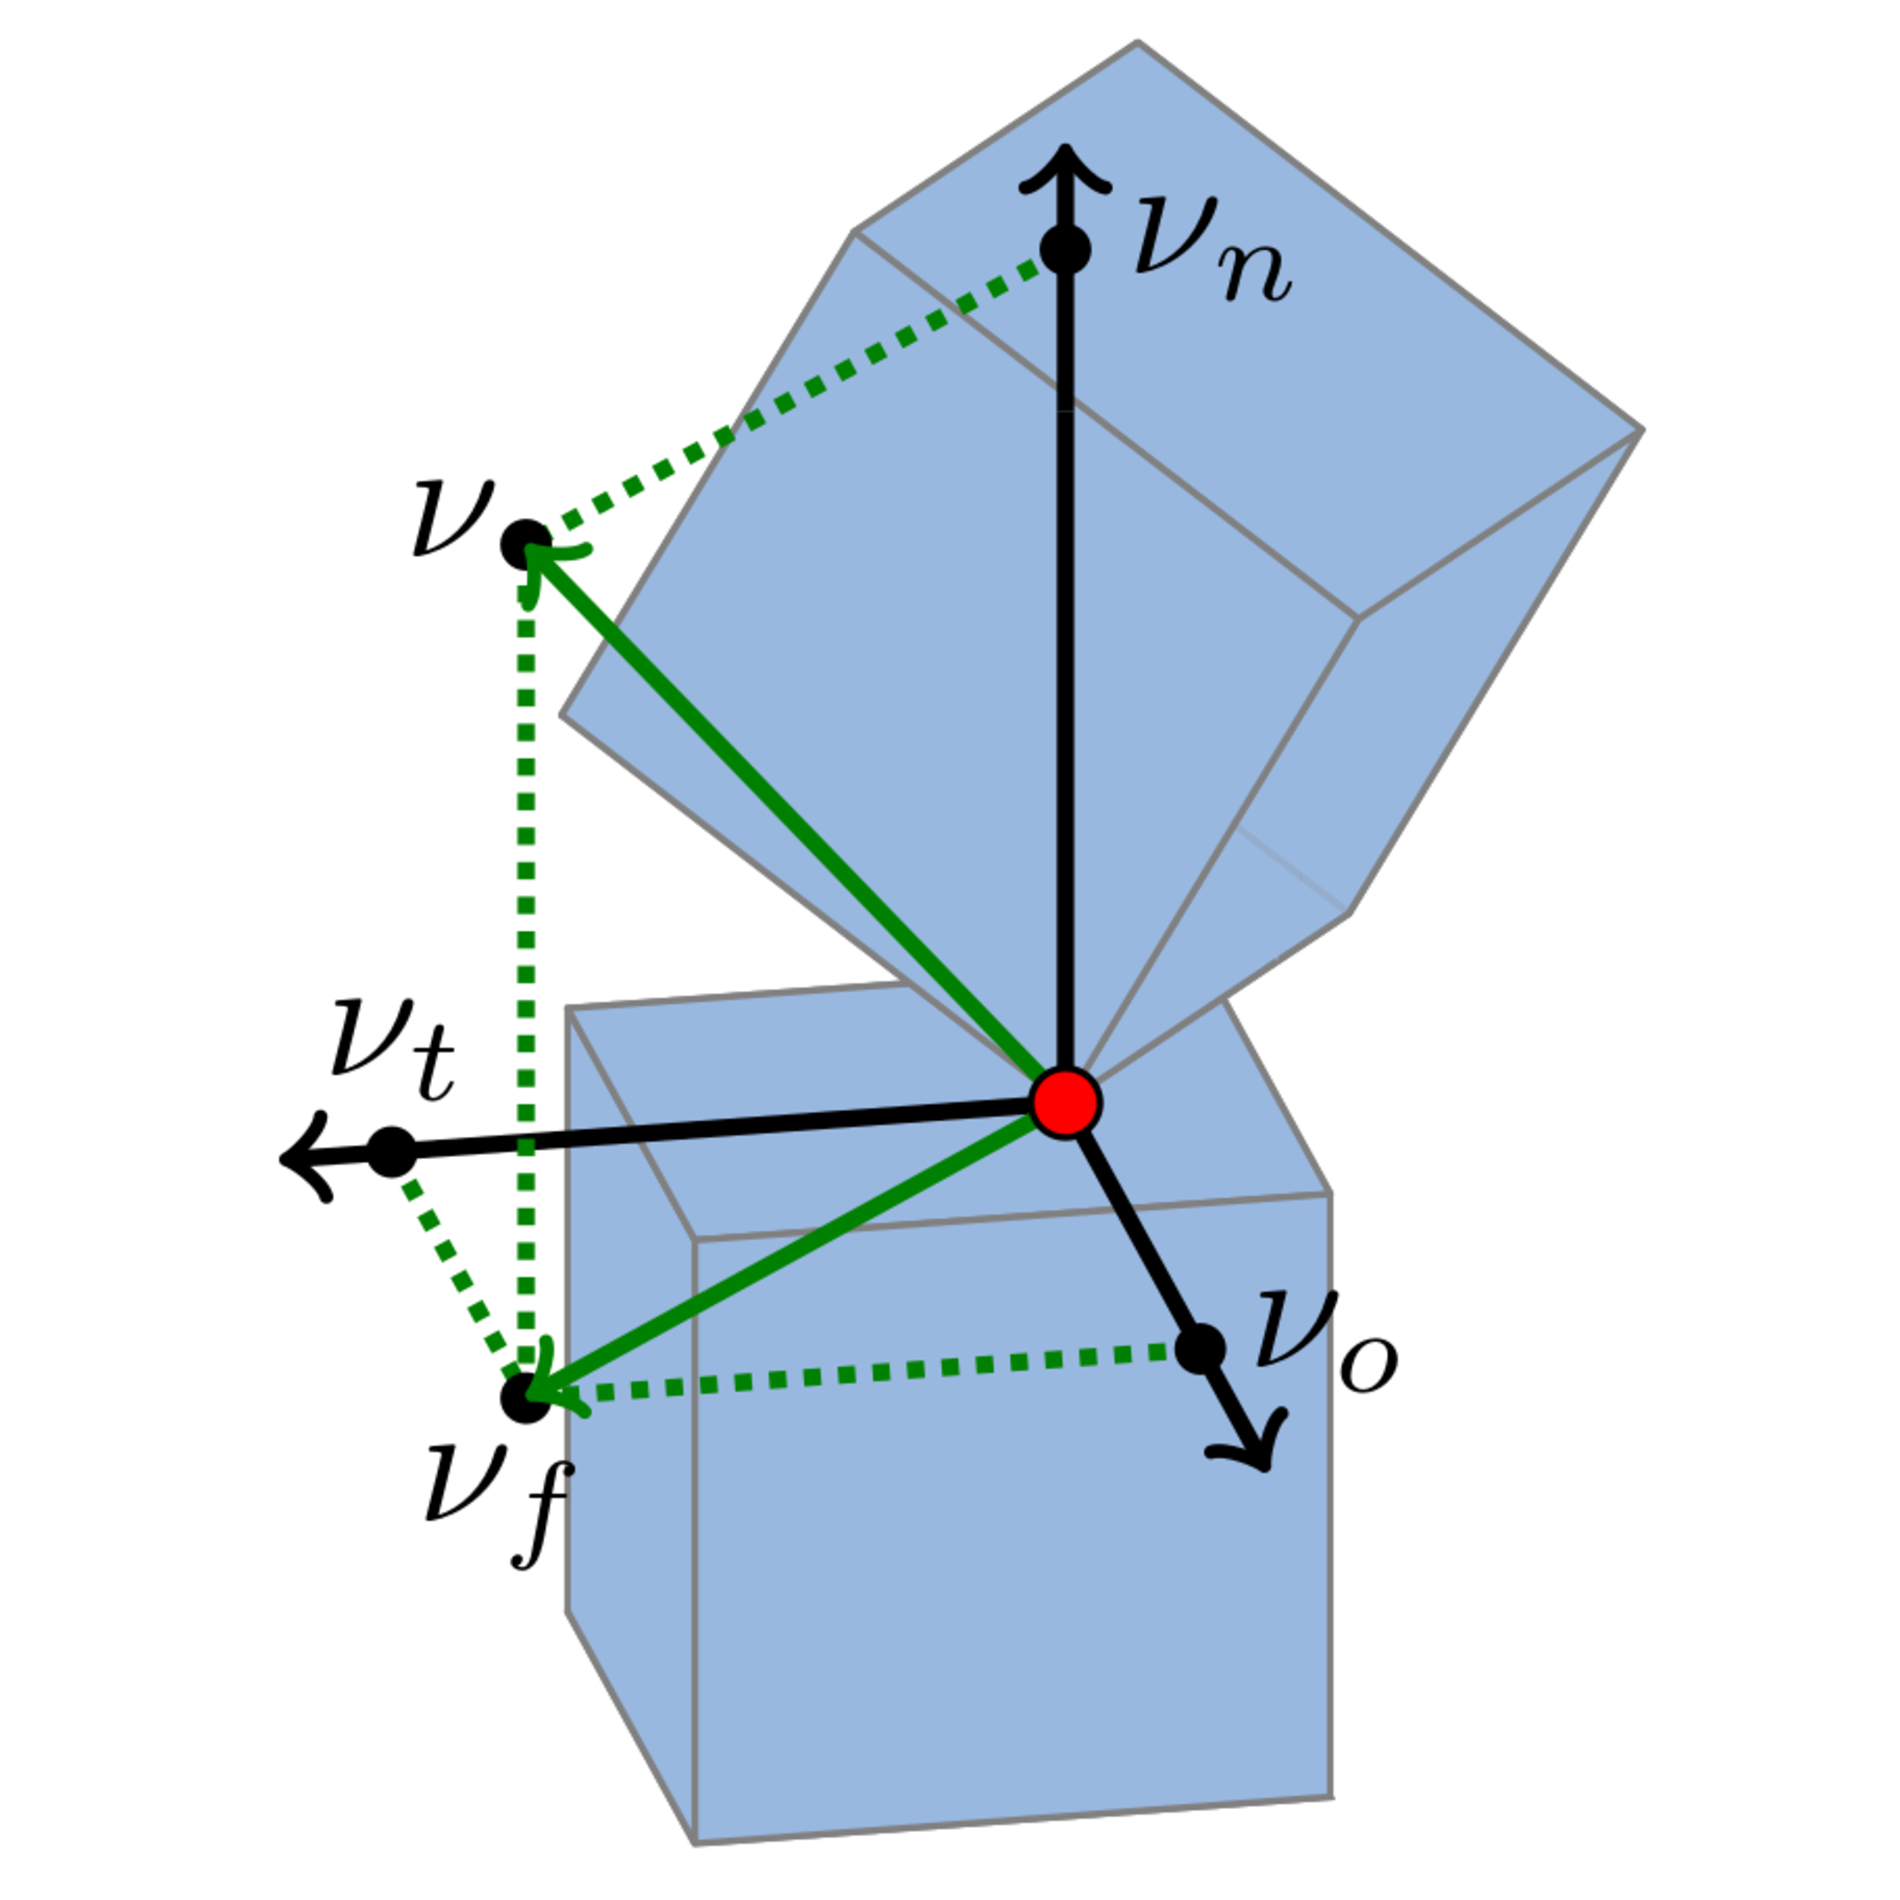
\includegraphics[width=\textwidth]{figures/friction_cube}
%	\caption{Contact velocities}
%	\label{fig:friction_cube}
%\end{subfigure}
%\caption[Friction cone and relative velocities]{Friction cone of a contact and decomposition of the contact force and relative velocity. Source: \cite{BETC2012}}
%\label{fig:ph}
%\end{figure}

\section{Simulation loop}
\Cref{fig:phase_simul} describes the main loop of a physics engine. A simulation step begins with the detection of collision points (Collision detection) which are then used to correct the positions of bodies to prevent interpenetration (Collision resolution) before being used to derive constraints to be incorporated in the complementarity problem (Contact handling), along with other active forces (gravity, or a motor generating torque). 

Finally, the CP is solved (Time integration) to determine the positions and velocities of the rigid bodies at the next time step and the loop begins anew.

\begin{figure}[htp]
\centering
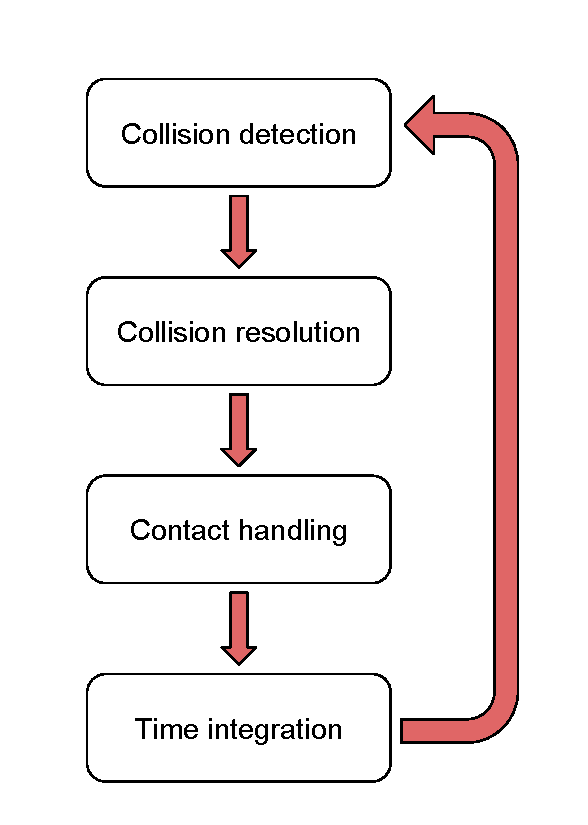
\includegraphics[width=0.5\textwidth]{figures/star_simul_loop2}
\caption[Modular phase description of the sub tasks of a rigid body simulator]{Modular phase description of the sub tasks of a rigid body simulator. Source: \cite{BETC2012}}
\label{fig:phase_simul}
\end{figure}